\documentclass[12pt,a4paper]{article}
\pdfoutput=1

\usepackage[utf8]{inputenc}
\usepackage[T1]{fontenc}
\usepackage[english]{babel}
\usepackage{amsmath}
\usepackage{lmodern}
\usepackage{units}
\usepackage{siunitx}
\usepackage{icomma}
\usepackage{color}
\usepackage{graphicx}
\usepackage{bbm}
\usepackage{transparent}
\newcommand{\N}{\ensuremath{\mathbbm{N}}}
\newcommand{\Z}{\ensuremath{\mathbbm{Z}}}
\newcommand{\Q}{\ensuremath{\mathbbm{Q}}}
\newcommand{\R}{\ensuremath{\mathbbm{R}}}
\newcommand{\C}{\ensuremath{\mathbbm{C}}}
\newcommand{\rd}{\ensuremath{\mathrm{d}}}
\newcommand{\id}{\ensuremath{\,\rd}}
\usepackage{hyperref}

\title{Time-Domain Reflectometry (TDR) using a Vector Network Analyzer (VNA)}
\author{Marcus Malmquist}
\date{\today}
\pagenumbering{gobble}

\begin{document}

\maketitle

\begin{abstract}
This report aims to present how a VNA was used to perform TDR on a few different circuits as well as an explanation of the results.
\end{abstract}

\newpage
\pagenumbering{roman}
\tableofcontents
\newpage
\pagenumbering{arabic}
\section{Introduction}
Time-domain Reflectometry is a method of performing measurements on transmission lines by sending a signal (typically a pulse or a voltage step) through it. The response from the transmission line can then studied to obtain information about some characteristics of the transmission line. These characteristics include cable length and termination.

One of the usages of TDR is that it can reveal if a cable is damaged or if a connection is poorly matched. This can be useful if the transmission line is located underground or otherwise difficult to access since the exact location of the damage can be obtained using TDR.

\section{Theory}\label{sec:theory}
In order to understand how TDR works it is necessary to understand the concepts of how an electromagnetic waves is transmitted and reflected at the interface between two materials. This will be done by introducing a reflection coefficient, $\Gamma$. Further reading on this subject can be done in \cite{cheng}.

\subsection{Reflection coefficient}\label{sec:refl}
Consider an electromagnetic wave $\vec{E}(\vec{r})$ (omitting the time-dependence). We want to use Ohm's law (\ref{eq:ohm}) to derive an expression for the reflection coefficient at an interface between two materials.
\begin{equation}
  \vec{J}=\sigma\vec{E}
  \label{eq:ohm}
\end{equation}
To simplify the derivation we introduce the voltage $V(\vec{r})$, current $I(\vec{r})$ and impedance $Z(\vec{r})$ from (\ref{eq:subs}) and end up with a version of Ohm's law more commonly used in circuit theory, $V=ZI$.
\begin{equation}
  \begin{array}{lll}
    I(\vec{r}) & = & \int_S \vec{J}(\vec{r})\cdot d\vec{S} \\
    V(\vec{r}) & = & \int_l \vec{E}(\vec{r})\cdot d\vec{l} \\
    Z(\vec{r}) & = & \sigma\frac{l}{S}
  \end{array}
  \label{eq:subs}
\end{equation}
We now introduce the voltage of the forward-moving wave, $V^{+}(\vec{r})$, and the backward-moving wave, $V^{-}(\vec{r})$ and define $\Gamma(\vec{r})$ such that
\begin{equation}
  V^{-}(\vec{r})=\Gamma(\vec{r}) V^{+}(\vec{r})
  \label{eq:gamma}
\end{equation}
The observed voltage wave would be the sum of the forward- and backward-moving wave, $V(\vec{r})=V^{+}(\vec{r})+V^{-}(\vec{r})$. Likewise the observed current wave would be the sum of the forward- and backward-moving wave, $I(\vec{r})=I^{+}(\vec{r})-I^{-}(\vec{r})$. Using Ohm's law and (\ref{eq:gamma}) yielding
\begin{equation}
  \begin{array}{lll}
    Z(\vec{r}) & = & \frac{V(\vec{r})}{I(\vec{r})} \\
         & = & \frac{V^{+}(\vec{r})+V^{-}(\vec{r})}{I^{+}(\vec{r})-I^{-}(\vec{r})} \\
         & = & Z_{0}\frac{V^{+}(\vec{r})+V^{-}(\vec{r})}{V^{+}(\vec{r})-V^{-}(\vec{r})} \\
         & = & Z_{0}\frac{1+\Gamma(\vec{r})}{1-\Gamma(\vec{r})}
  \end{array}
  \label{eq:z}
\end{equation}
In some cases it can be useful to rewrite (\ref{eq:z}) as
\begin{equation}
  \Gamma(\vec{r})=\frac{Z(\vec{r})-Z_{0}}{Z(\vec{r})+Z_{0}}
  \label{eq:gamma_2}
\end{equation}

In the time domain the response for higher frequency components of the signal will be displayed first and the lower frequency components later. This means that information about how the load responds to different frequencies can be collected from the response.


\subsection{Reflections in unmatched circuits}\label{sec:unmatched}
If a circuit consists of several unmatched interfaces we have to make some changes to the calculations from \ref{sec:refl}. The forward- and backward-moving wave is now a superposition of several forward- and backward-moving waves.
\begin{equation}
  \begin{array}{lll}
    V(\vec{r}) & = & \displaystyle\sum_{i}(V^{+}_{i}+V^{-}_{i}) \\
    I(\vec{r})& = & \displaystyle\sum_{i}(I^{+}_{i}-I^{-}_{i})
  \end{array}
\end{equation}
With this change (\ref{eq:z}) becomes (\ref{eq:z_new}).
\begin{equation}
  \begin{array}{lll}
    Z(\vec{r}) & = & \frac{V(\vec{r})}{I(\vec{r})} \\
               & = & \frac{\sum_{i}(V^{+}_{i}+V^{-}_{i})}{\sum_{i}(I^{+}_{i}-I^{-}_{i})} \\
               & = & Z_{0}\frac{\sum_{i}(V^{+}_{i}+V^{-}_{i})}{\sum_{i}(V^{+}_{i}-V^{-}_{i})} \\
     & = & Z_{0}\frac{1+\sum_{i}(\prod_{j}\Gamma_{j}(\vec{r})\prod_{k}(1+\Gamma_{k}(\vec{r})))}{1-\sum_{i}(\prod_{j}\Gamma_{j}(\vec{r})\prod_{k}(1+\Gamma_{k}(\vec{r})))}
  \end{array}
  \label{eq:z_new}
\end{equation}
It should be noted that if $Z(\vec{r})$ is comprised of many components that are of interest it may be easier to measure $\prod_{j}\Gamma_{j}(\vec{r})\prod_{k}(1-\Gamma_{k}(\vec{r}))$ for the corresponding $i$ and solve for the $\Gamma_{j}$ (or $\Gamma_{k}$) of interest and then use that in (\ref{eq:z}) and solve recursively to get the individual components rather than solving (\ref{eq:z_new}).

\subsection{Length of transmission line}
The length of a transmission line can be calculated by measuring the time it takes before the response returns at which point the signal has travelled twice the length of the cable. The length can then be calculated if the propagation velocity in the cable is known.
\begin{equation}
  l=c\frac{t_{2l}}{2}=\frac{c_{0}}{\sqrt{\mu_{\text{r}}\epsilon_{\text{r}}}}\frac{t_{2l}}{2}
  \label{eq:cablen}
\end{equation}

\section{Equipment}\label{sec:equip}
Below follows a list of the equipment used in the lab exercise. The VNA was connected to the black boxes via a coaxial cable. The VNA was set to display the real part of the signal and as such it displayed the reflection coefficient for the DC part of the signal. The $x$-axis was set to display the length of the cable calibrated from the end of the coaxial cable attached to the VNA.
\begin{itemize}
\item VNA (Vector Network Analyzer)
\item Coaxial cable ($Z_{0}=\SI{50}{\ohm}$)
\item Black box \#1
  \begin{itemize}
  \item Short-circuit termination
  \item Open-circuit termination
  \item Purely resistive loads
  \end{itemize}
\item Black box \#2 (II-B)
  \begin{itemize}
  \item Unmatched transmission line ($Z_{0}\neq\SI{50}{\ohm}$)
  \item Load
  \end{itemize}
\item Black box \#3
  \begin{itemize}
  \item Matched transmission line ($Z_{0}=\SI{50}{\ohm}$)
  \item Load
  \end{itemize}
\end{itemize}
The VNA needs to be set according to \cite{labpm}:
\begin{itemize}
\item MEAS
  \begin{itemize}
  \item S11, balanced
  \item Ports: P1
  \end{itemize}
\item TRACE CONFIG
  \begin{itemize}
  \item Type: Low Pass Step
  \item Time domain
  \end{itemize}
\item FORMAT
  \begin{itemize}
  \item Real
  \end{itemize}
\item SCALE
  \begin{itemize}
  \item max = 1 U
  \item min = -1 U
  \end{itemize}
\item START
  \begin{itemize}
  \item Stimulus
  \end{itemize}
\item STOP
  \begin{itemize}
  \item Stimulus 5 GHz
  \end{itemize}
\item SWEEP
  \begin{itemize}
  \item Number of points: 499
  \item Freq step: 10 MHz
  \end{itemize}
\item OFFSET EMBED
  \begin{itemize}
  \item Velocity factor: 0.66
  \end{itemize}
\end{itemize}

\section{Method}
The lab exercise was divided into three different tasks. These tasks involved determining the type of termination of a transmission line and the length of the transmission line for a matched and unmatched circuit. The VNA was set according to the settings in \ref{sec:equip} unless the cable length was too long (which was the case in Black box \#3) in which case the stop stimulus was lowered.

\subsection{Black box \#1, Study known terminations}
The coaxial cable was terminated with the terminations described in \ref{sec:equip}. The reflection coefficient, $\Gamma$, was measured on the VNA and used in (\ref{eq:gamma_2}) to find the value of the loads.

\subsection{Black box \#2, Study unknown unmatched circuit}
The black box was connected to the VNA and the response was displayed. Measurements were conducted once the response was stable. Using the information in \ref{sec:unmatched} the parameters in Figure~\ref{fig:iib} could be calculated.

\begin{figure}[ht]
  \centering
  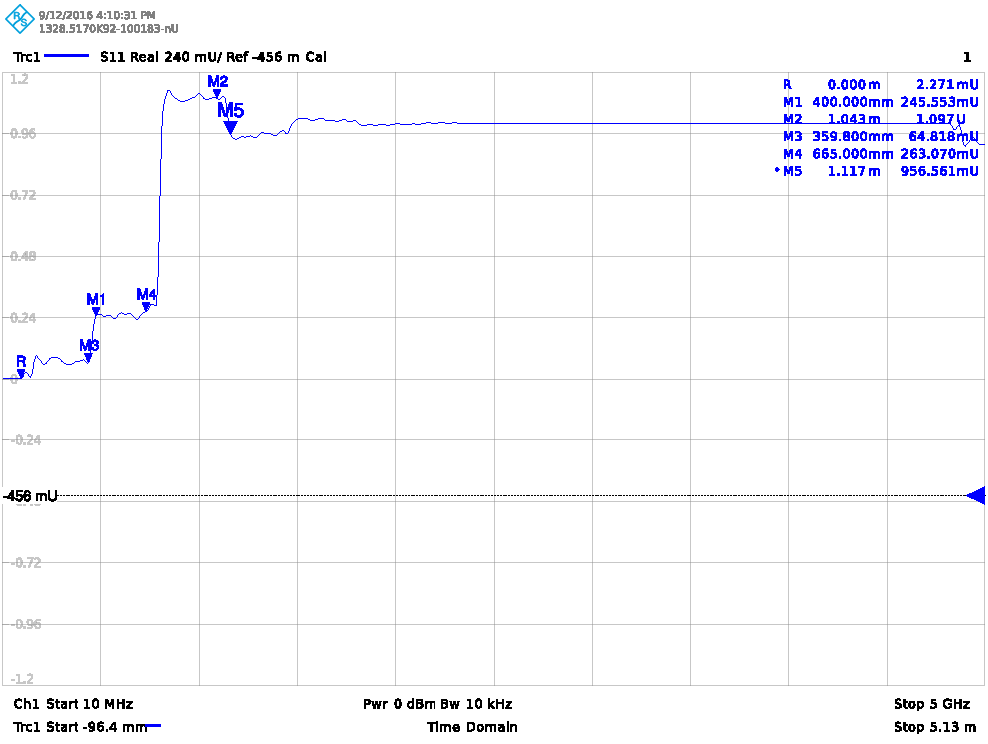
\includegraphics[width=\textwidth]{II-B_SVG.pdf}
  \caption{\label{fig:iib} A schematic image of the black box \#2 (II-B).}
\end{figure}

\subsection{Black box \#3, Study unknown matched circuit}
The black box was comprised of four coaxial cables of unknown length and each with a different termination was connected to the VNA and the response displayed. The type of termination could be determined by looking at the response for the high frequencies as well as the low frequencies as explained in \ref{sec:refl}.

\section{Results}
The results presented in this section was achieved by measuring the reflected signal using the built-in markers in the VNA and use the values extracted from the markers in the equations from \ref{sec:theory}.
\subsection{Black box \#1, Study known terminations}
The relevant measurements on the black box can be seen in Table~\ref{tab:box1}, where the reflection coefficients were found by measuring the output on the display of the VNA and the value of the resistors were found by using (\ref{eq:z}).
\begin{table}[ht]
  \centering
  \caption{Measured data from black box \#1 and the values of the components causing the reflections.}
  \begin{tabular}{|l|r|}\hline
    $\Gamma_{\text{open}}$ & $1$ \\
    $\Gamma_{\text{short}}$ & $-1$ \\
    $\Gamma_{R_{1}}$ & $-0.23$ \\
    $R_{1}$ & $\SI{30}{\ohm}$ \\
    $\Gamma_{R_{2}}$ & $0.33$ \\
    $R_{2}$ & $\SI{100}{\ohm}$ \\ \hline
  \end{tabular}
  \label{tab:box1}
\end{table}
\subsection{Black box \#2, Study unknown unmatched circuit}
The reflected signal as it was seen on the VNA monitor can be seen in Figure~\ref{fig:response}. To facilitate the calculations leading to finding the values of the variables depicted in Figure~\ref{fig:iib}, one can create a schematic image of how the signal propagates in the black box. This can be seen in Figure~\ref{fig:iibrefl} and from it a set of equations can be modelled.
\begin{equation}
  \begin{cases}
    \Gamma_{1}=0.20 \\
    \Gamma_{2}(1-\Gamma_{1}^{2})=0.84 \\
    l=\SI{360}{\milli\metre}
  \end{cases}
\end{equation}
Solving these for $\Gamma_{1}$, $\Gamma_{2}$ and $l$ and use these in (\ref{eq:z}) yields the values presented in Table~\ref{tab:box2_res}.
\begin{table}[ht]
  \centering
  \caption{The values of the variables in black box \#2 calculated from the measured data.}
  \begin{tabular}{|l|r|}\hline
    $l$ & $\SI{360}{\milli\metre}$ \\
    $R_{02}$ & $\SI{75}{\ohm}$ \\
    $R_{L}$ & $\SI{860}{\ohm}$ \\ \hline
  \end{tabular}
  \label{tab:box2_res}
\end{table}

\begin{figure}[ht]
  \centering
  \input{II-B-refl.pdf_t}
  \caption{\label{fig:iibrefl} A schematic image of the signal propagating in black box \#2 (II-B).}
\end{figure}

\begin{figure}[ht]
  \centering
  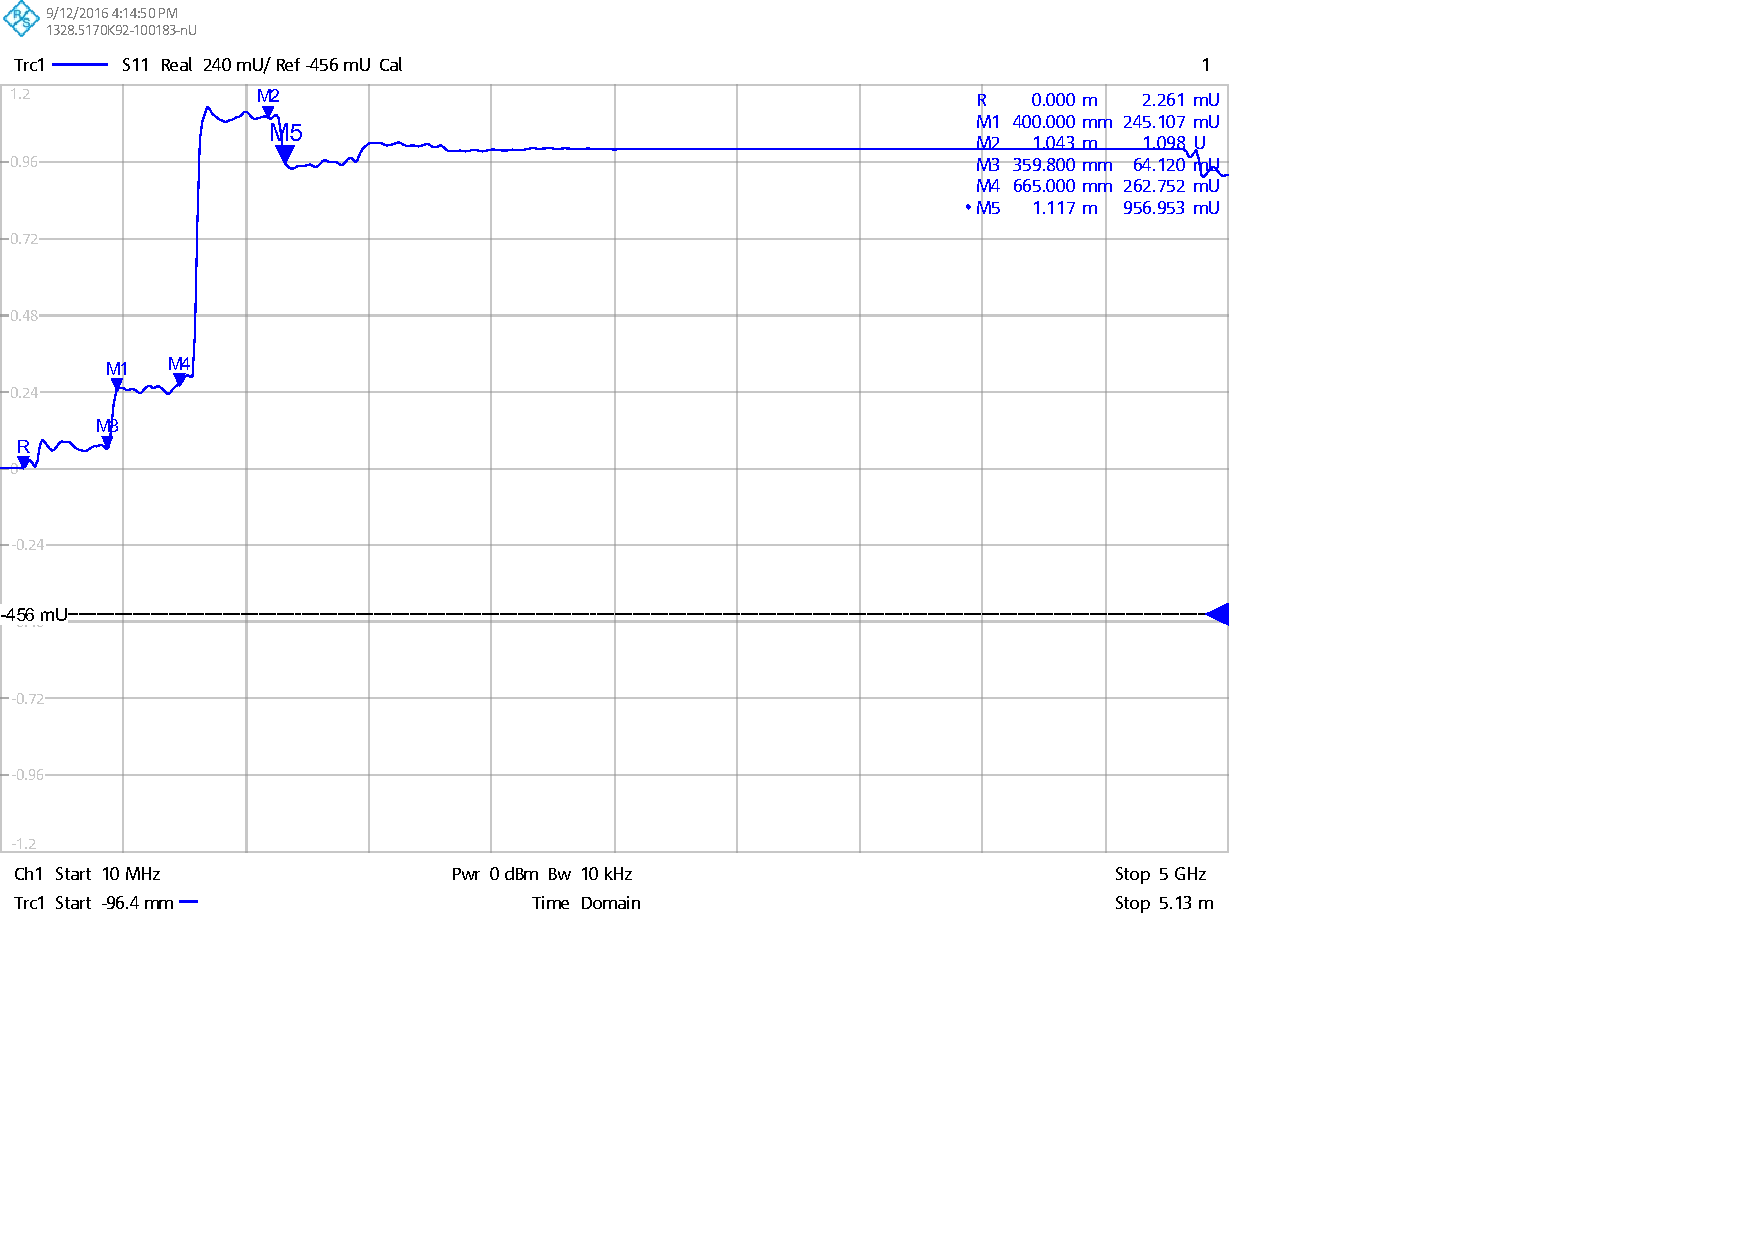
\includegraphics[width=\textwidth]{Han_Marcus_II-B.pdf}
  \caption{\label{fig:response} The step response from black box \#2 (II-B).}
\end{figure}

\subsection{Black box \#3, Study unknown matched circuit}
The black box was comprised of 4 different ports (A, B, C and D).

Port A was terminated such that $\Gamma=1$ after $\SI{0.4}{\metre}$ indicating that it was terminated in an open circuit.

Port B was terminated such that it acted as an open circuit for high frequencies and a very small resistor for low frequencies indicating that it was terminated in an inductor in series with a resistor ($R\ll Z_0$). It was terminated after $\SI{2.0}{\metre}$.

The termination of port C acted as an open circuit for high frequencies and a resistor for low frequencies indicating that is was terminated in an inductor in series with a resistor ($R<Z_{0}$). The transmission line was $\SI{0.75}{\metre}$.

The termination of port D acted as a short circuit for high frequencies and an open circuit for low frequencies indicating that it was terminated in a capacitor. The transmission line was $\SI{9.5}{\metre}$.

\section{Discussion and conclusion}
The measurements were pretty straight forward and not much ambiguity in the measurements as the step responses did not change much on the monitor. We did not reconnect the black boxes a few time to ensure that our result was as accurate as possible which in hindsight would have been good. One exception from this was the black box \#2 which gave a response that jittered alot so there is likely some considerable uncertainty in the calculated values of the resistors (in particular $R_{L}$ where it is only safe to say that $R_{L}\gg R_{02}$ and $R_{L}\sim\SI{1}{\kilo\ohm}$).

An observation made about black box \#3 port B is that the step response looks very similar to a coaxial cable split into two parallel cables which are then terminated in a short circuit, (perhaps in an attempt to simulate a short circuit termination). The reason this could be true is that the inductance and resistance appeared to be very small for the termination, which would be the case if the coaxial cable was terminated as previously explained.

\newpage
\begin{thebibliography}{1}

\bibitem{labpm} H. Hjelmgren. ``Time Domain Reflectometry (TDR) using a Vector Network Analyzer (VNA).'' Internet: \url{https://pingpong.chalmers.se/courseId/7038/node.do?id=3211479&ts=1473400633515&u=-1631444947}, 2016-09-09 [2016-10-09]

\bibitem{cheng} D. K. Cheng. ``Theory and Applications of Transmission Lines'' in \textit{Field and Wave Electromagnetics}, 2$^{\text{nd}}$ ed. Edinburgh: Pearson, 2014, pp. 427-519

\end{thebibliography}

\end{document}
